\documentclass[11pt]{article}

\usepackage{times}
\usepackage{epsf}
\usepackage{epsfig}
\usepackage{amsmath, alltt, amssymb, xspace}
\usepackage{wrapfig}
\usepackage{fancyhdr}
\usepackage{url}
\usepackage{verbatim}
\usepackage{fancyvrb}
\usepackage{float}

\usepackage{subfigure}
\usepackage{cite}
\usepackage{hyperref}
\hypersetup{%
    pdfborder = {0 0 0}
}
\topmargin      -0.50in  % distance to headers
\oddsidemargin  0.0in
\evensidemargin 0.0in
\textwidth      6.5in
\textheight     8.9in


%\centerfigcaptionstrue

%\def\baselinestretch{0.95}


\newcommand\discuss[1]{\{\textbf{Discuss:} \textit{#1}\}}
%\newcommand\todo[1]{\vspace{0.1in}\{\textbf{Todo:} \textit{#1}\}\vspace{0.1in}}
\newtheorem{problem}{Problem}[section]
%\newtheorem{theorem}{Theorem}
%\newtheorem{fact}{Fact}
\newtheorem{define}{Definition}[section]
%\newtheorem{analysis}{Analysis}
\newcommand\vspacenoindent{\vspace{0.1in} \noindent}

%\newenvironment{proof}{\noindent {\bf Proof}.}{\hspace*{\fill}~\mbox{\rule[0pt]{1.3ex}{1.3ex}}}
%\newcommand\todo[1]{\vspace{0.1in}\{\textbf{Todo:} \textit{#1}\}\vspace{0.1in}}

%\newcommand\reducespace{\vspace{-0.1in}}
% reduce the space between lines
%\def\baselinestretch{0.95}

\newcommand{\fixmefn}[1]{ \footnote{\sf\ \ \fbox{FIXME} #1} }
\newcommand{\todo}[1]{
\vspace{0.1in}
\fbox{\parbox{6in}{TODO: #1}}
\vspace{0.1in}
}

\newcommand{\mybox}[1]{
\vspace{0.2in}
\noindent
\fbox{\parbox{6.5in}{#1}}
\vspace{0.1in}
}


\newcounter{question}
\setcounter{question}{1}

\newcommand{\myquestion} {{\vspace{0.1in} \noindent \bf Question \arabic{question}:} \addtocounter{question}{1} \,}

\newcommand{\myproblem} {{\noindent \bf Problem \arabic{question}:} \addtocounter{question}{1} \,}



\newcommand{\copyrightnotice}[1]{
\vspace{0.1in}
\fbox{\parbox{6in}{
			This lab was developed by Sparta Global for Cybersecurity courses.
			It was built based on the original lab that was developed for the Labtainer framework by the Naval Postgraduate School, Center for Cybersecurity and Cyber Operations under National Science Foundation Award No. 1438893.
      This work is in the public domain, and cannot be copyrighted.
			}}
\vspace{0.1in}
}


\newcommand{\idea}[1]{
\vspace{0.1in}
{\sf IDEA:\ \ \fbox{\parbox{5in}{#1}}}
\vspace{0.1in}
}

\newcommand{\questionblock}[1]{
\vspace{0.1in}
\fbox{\parbox{6in}{#1}}
\vspace{0.1in}
}


\newcommand{\argmax}[1]{
\begin{minipage}[t]{1.25cm}\parskip-1ex\begin{center}
argmax
#1
\end{center}\end{minipage}
\;
}

\newcommand{\bm}{\boldmath}
\newcommand  {\bx}    {\mbox{\boldmath $x$}}
\newcommand  {\by}    {\mbox{\boldmath $y$}}
\newcommand  {\br}    {\mbox{\boldmath $r$}}


\newcommand{\tstamp}{\today}
%\rfoot[\fancyplain{\tstamp} {\tstamp}]  {\fancyplain{}{}}

\pagestyle{fancy}
\lhead{\bfseries Labtainers}
\chead{}
\rhead{\small \thepage}
\lfoot{\small{\textit{Dr. Osama Abu Oun - Cybersecurity Courses - Sparta Global (\url{https://www.spartaglobal.com/})}}}
\cfoot{}
\rfoot{}

\begin{document}

\begin{center}
{\LARGE Firewall/IPTables - Lab Guide}
\vspace{0.1in}\\
\end{center}

\copyrightnotice

\section{Overview}
Iptables is a command line software-based firewall in Linux. It uses policy chains to allow and to block traffic.

IPTables is used as a Firewall and can perform NAT and PAT operations.

In this lab, we focus on IPTables configuration to allow and deny access from/to IP addresses and/or services.

\section{Lab Environment}
This lab runs in the Labtainer framework,
available at http://my.nps.edu/web/c3o/labtainers.
That site includes links to a pre-built virtual machine
that has Labtainers installed, however Labtainers can
be run on any Linux host that supports Docker containers.

From your labtainer-student (~/labtainer/labtainer-student) directory start the lab using:
\begin{verbatim}
    labtainer sparta-firewall
\end{verbatim}
\noindent A link to this lab guide will be displayed.

\section{Network Configuration}
IP addresses and routing are configured on all devices.

\begin{figure}[H]
\begin{center}
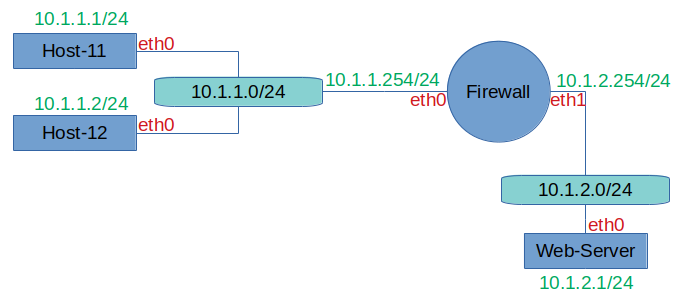
\includegraphics [width=0.8\textwidth]{labtainers-firewall-lab-01.png}
\end{center}
\caption{Network topology for routing-basics lab}
\label{fig:topology}
\end{figure}

\section{Credentials}
\begin{itemize}
	\item \textbf{Host-11}:
	\begin{itemize}
		\item \textbf{Username:} user-11
		\item \textbf{Password:} user-11
	\end{itemize}
	\item \textbf{Host-12}:
	\begin{itemize}
		\item \textbf{Username:} user-12
		\item \textbf{Password:} user-12
	\end{itemize}o
	\item \textbf{Web-Server}:
	\begin{itemize}
		\item \textbf{Username:} web-admin
		\item \textbf{Password:} web-admin
	\end{itemize}
	\item \textbf{Firewall}:
	\begin{itemize}
		\item \textbf{Username:} admin
		\item \textbf{Password:} admin
	\end{itemize}
\end{itemize}

\section{Lab Tasks}

\subsection{Testing the Initial Configuration}\label{Testing the Initial Configuration}
Lets check what can/can't we do in this network.
\newline
\begin{itemize}
	\item On Host-11 (Ping Host-11 -$>$ Web-Server)
	\begin{verbatim}
	    ping 10.1.2.1
	\end{verbatim}

	What is the result ?
	\item On Host-11 (Send HTTP request Host-11 -$>$ Web-Server to get a web page)
	\begin{verbatim}
	    wget http://10.1.2.1/index.html
	\end{verbatim}

	What is the result ?
	\item On Host-11 (SSH Access Host-11 -$>$ Router1 to access the server itself)
	\begin{verbatim}
	    ssh web-admin@10.1.2.1
	\end{verbatim}

	\textbf{Note:} You will be prompted to accept adding the SSH fingerprint
	\newline
	The authenticity of host '10.1.2.1 (10.1.2.1)' can't be established.
	ECDSA key fingerprint is SHA256:Z2/CHKW/UJw7HHi2r73gtKOO2cUFNxs2K6io3sMMGIQ.
	Are you sure you want to continue connecting (yes/no)?
	You should type `yes` and hit `Enter`. In a real environment, you need to check whether the fingerprint is correct or not in order to prevent some types of attacks against SSH protocol (this subject will be discussed later in Cybersecurity module).
	\newline
	\newline
	\textbf{Note:} Be patient, it takes long time to start.
	\newline
	\newline
	What is the result ?
	\item On Host-12 (Ping Host-12 -$>$ Router1)
	\begin{verbatim}
	    ping 10.1.1.254
	\end{verbatim}

	What is the result ?

	\item On Host-12 (Ping Host-12 -$>$ Web-Server)
	\begin{verbatim}
	    ping 10.1.2.1
	\end{verbatim}

	What is the result ?
	\item On Host-12 (Send HTTP request Host-12 -$>$ Web-Server to get a web page)
	\begin{verbatim}
	    wget http://10.1.2.1/index.html
	\end{verbatim}

	What is the result ?
	\item On Host-12 (SSH Access Host-12 -$>$ Router1 to access the server itself)
	\begin{verbatim}
	    ssh web-admin@10.1.2.1
	\end{verbatim}

	\textbf{Note:} Accept the SSH fingerprint
	\newline
	\newline
	What is the result ?
	\item On Host-12 (Ping Host-12 -$>$ Router1)
	\begin{verbatim}
	    ping 10.1.1.254
	\end{verbatim}

	What is the result ?
\end{itemize}

\subsection{Configuring the Firewall}

Now, lets configure the firewall to allow only:
\begin{itemize}
	\item Host-11 -$>$ Web-Server: SSH Protocol (TCP 22)
	\item Host-12 -$>$ Web-Server: HTTP Protocol (TCP 80)
\end{itemize}

\textbf{The default rules in iptables allow all type of traffic to pass.}

\begin{itemize}
	\item We will start by deleting (flushing) all rules.
	\begin{verbatim}
			sudo iptables -F
			sudo iptables -t nat -F
			sudo iptables -X
	\end{verbatim}

	\item Drop all packets by default
	\begin{verbatim}
			sudo iptables -P FORWARD DROP
			sudo iptables -P INPUT   DROP
			sudo iptables -P OUTPUT  DROP
	\end{verbatim}

	\item Allow (Operation: ACCEPT) forwarding traffic on firewall that matches the rules:
		\begin{itemize}
			\item Source IP: 10.1.1.1
			\item Destination IP: 10.1.2.1
			\item	Protocol: TCP
			\item Port: 22 (SSH)
		\end{itemize}
		\begin{verbatim}
				sudo iptables -A FORWARD -p tcp --dport 22 -s 10.1.1.1 -d 10.1.2.1 -j ACCEPT
		\end{verbatim}

		\item On Host-11 (SSH Access Host-11 -$>$ Router1 to access the server itself)
		\begin{verbatim}
		    ssh web-admin@10.1.2.1
		\end{verbatim}

		What is the result ? What is the reason in your opinion ?

		\item Allow (Operation: ACCEPT) forwarding traffic on firewall that matches the rules:
			\begin{itemize}
				\item Source IP: 10.1.1.2
				\item Destination IP: 10.1.2.1
				\item	Protocol: TCP
				\item Port: 80 (HTTP)
			\end{itemize}
			\begin{verbatim}
					sudo iptables -A FORWARD -p tcp --dport 80 -s 10.1.1.2 -d 10.1.2.1 -j ACCEPT
			\end{verbatim}

			\item Test the connectivity: On Host-12 (Send HTTP request Host-12 -$>$ Web-Server to get a web page)
			\begin{verbatim}
			    wget http://10.1.2.1/index.html
			\end{verbatim}

			What is the result ? What is the reason in your opinion ?

		\item allow the traffic that it is a part of a connection to pass through the firewall
		\begin{verbatim}
				sudo iptables  -A FORWARD -m conntrack --ctstate ESTABLISHED,RELATED -j ACCEPT
		\end{verbatim}
\end{itemize}

Now, refer to Section \ref{Testing the Initial Configuration} and redo all the tests again. Report to your instructor the tests which they worked and the ones that didn't work.


\section{Submission}
After finishing the lab, go to the terminal on your Linux system that was used to start the lab and type:
\begin{verbatim}
    stoplab sparta-firewall
\end{verbatim}
When you stop the lab, the system will display a path to the zipped lab results on your Linux system.  Provide that file to
your instructor, e.g., via the Sakai site.

\end{document}
